\documentclass{rosenpass-beamer}

\usepackage[british,UKenglish,USenglish,english,german]{babel}
\usepackage[autostyle]{csquotes}
\usepackage{emoji}
\let\say\enquote

\usepackage{xurl}

\urlstyle{same}

\usepackage{textcomp}

\usetikzlibrary{positioning,decorations.pathreplacing,svg.path}

\definecolor{RPPink}{rgb}{274,4,132}
\definecolor{RPOrange}{rgb}{255, 166, 48}
\definecolor{RPAquamarine}{rgb}{255, 166, 48}
\definecolor{RPLightGray}{rgb}{160, 159, 164}
\definecolor{RPTurquoise}{rgb}{114, 161, 229}

\title{Rosenpass}
\subtitle{PQC Wireguard as a new VPN}
\author{
Philip Kastura-Sahl
}
\institute{Universität Heidelberg}

\conference{IT-Security Seminar}
\date{18-01-2024}

\parskip\smallskipamount

\ExplSyntaxOn
\newcommand*{\sourcename}{Source}
\newcommand*{\sourcesep}{:~}
\newcommand*{\ImgSource}[2]{

\hbox_set:Nn \l_tmpa_box {#1}

\hbox_set:Nn \l_tmpa_box {
\dim_set:Nn \l_tmpa_dim {\box_ht:N \l_tmpa_box}
\hbox_unpack_drop:N \l_tmpa_box \rotatebox{90}{\parbox{\l_tmpa_dim}{\tiny\sourcename\sourcesep#2}}
}
\box_use:N \l_tmpa_box
}
\ExplSyntaxOff

% reduce itemize indent
\setlength{\leftmargini}{0pt}

\usepackage{biblatex}
\addbibresource{sources.bib}
\renewcommand*{\bibfont}{\scriptsize}

% namePartPictureSetup
\ExplSyntaxOn
\int_new:N \l__ptxcd_namepart_int
\fp_new:N \l__ptxcd_namepos_fp
\def\namepartsep{1.1}
\dim_new:N \l__ptxcd_namepart_sep_dim
\dim_set:Nn \l__ptxcd_namepart_sep_dim  {3mm}

\newcommand*{\namepart}[2][0]{
	\int_set:Nn \l__ptxcd_namepart_int {\clist_count:n {#2}}
	\begin{scope}[xshift=#1]
	\fp_set:Nn \l__ptxcd_namepos_fp {\l__ptxcd_namepart_int / 2}
	\keyval_parse:nnn {\__ptxcd_namepart_item:nn {}}{ \__ptxcd_namepart_item:nn } {#2}
	\end{scope}
}

\newcommand*{\SingleNamePart}[4][0]{
		\node[rounded~corners,fill=rosenpass-lightblue] (#2) at (#1,-.7) {\ttfamily#3};
		\node[above] at (#2.north) {\footnotesize #4};
}

\cs_new:Nn \__ptxcd_namepart_item:nn {
	\fp_sub:Nn \l__ptxcd_namepos_fp {1}
	\node[rounded~corners,fill=rosenpass-lightblue] (#1) at (0,\fp_use:N \l__ptxcd_namepos_fp * \namepartsep) {\ttfamily#1};
	\node[above] at (#1.north) {\footnotesize #2};
}


\newcommand*{\namebraceleft}[2] {
	\draw[decorate]([xshift=-\l__ptxcd_namepart_sep_dim]#2.south~west)--([xshift=-\l__ptxcd_namepart_sep_dim]#1.north~west) ;
}

\newcommand*{\namebraceright}[2]{
	\draw[decorate]([xshift=\l__ptxcd_namepart_sep_dim]#1.north~east) --([xshift=\l__ptxcd_namepart_sep_dim]#2.south~east);
}
\ExplSyntaxOff

\graphicspath{{}{graphics/}}

\begin{document}

\maketitle

%%%%%%%%%%%%%%%%%%%%%%%%%%%%%%%%%%%%%%%%%%%%%%%%%%%%%%%%%%%%%%%%%%%%%%%%%%%%%%%%%%%%%%%%%%%%%%%%%%%%%%%%%%%%%%%%%%%%%%%%%%%%%%%%%%%%%%%%%%%%%%%%%%%%%%%%%%%%%%%%%%%%%%%
% Begin Document
%%%%%%%%%%%%%%%%%%%%%%%%%%%%%%%%%%%%%%%%%%%%%%%%%%%%%%%%%%%%%%%%%%%%%%%%%%%%%%%%%%%%%%%%%%%%%%%%%%%%%%%%%%%%%%%%%%%%%%%%%%%%%%%%%%%%%%%%%%%%%%%%%%%%%%%%%%%%%%%%%%%%%%%

\begin{frame}{Wireguard\cite{wireguard}}
\begin{itemize}
  \item Handshake every two minutes
  \item Handshake based on Diffie-Hellman
  \item Uses pre-Quantumn ciphers
\end{itemize}
\end{frame}

%%%%%%%%%%%%%%%%%%%%%%%%%%%%%%%%%%%%%%%%%%%%%%%%%%%%%%%%%%%%%%%%%%%%%%%%%%%%%%%%%%%%%%%%%%%%%%%%%%%%%%%%%%%%%%%%%%%%%%%%%%%%%%%%%%%%%%%%%%%%%%%%%%%%%%%%%%%%%%%%%%%%%%%

\begin{frame}{Rosenpass\cite{rosenpass}\cite{cryptoeprint:2020/379}}
\begin{itemize}
  \item Post-quantum Encryption/Decryption in the wild!
  \item Spiritual Successor to PQ Wireguard
  \item Why?
  Because store now, decrypt later.
\end{itemize}
\end{frame}

%%%%%%%%%%%%%%%%%%%%%%%%%%%%%%%%%%%%%%%%%%%%%%%%%%%%%%%%%%%%%%%%%%%%%%%%%%%%%%%%%%%%%%%%%%%%%%%%%%%%%%%%%%%%%%%%%%%%%%%%%%%%%%%%%%%%%%%%%%%%%%%%%%%%%%%%%%%%%%%%%%%%%%%

\begin{frame}{Huh?\cite{openssl-documentation}}
  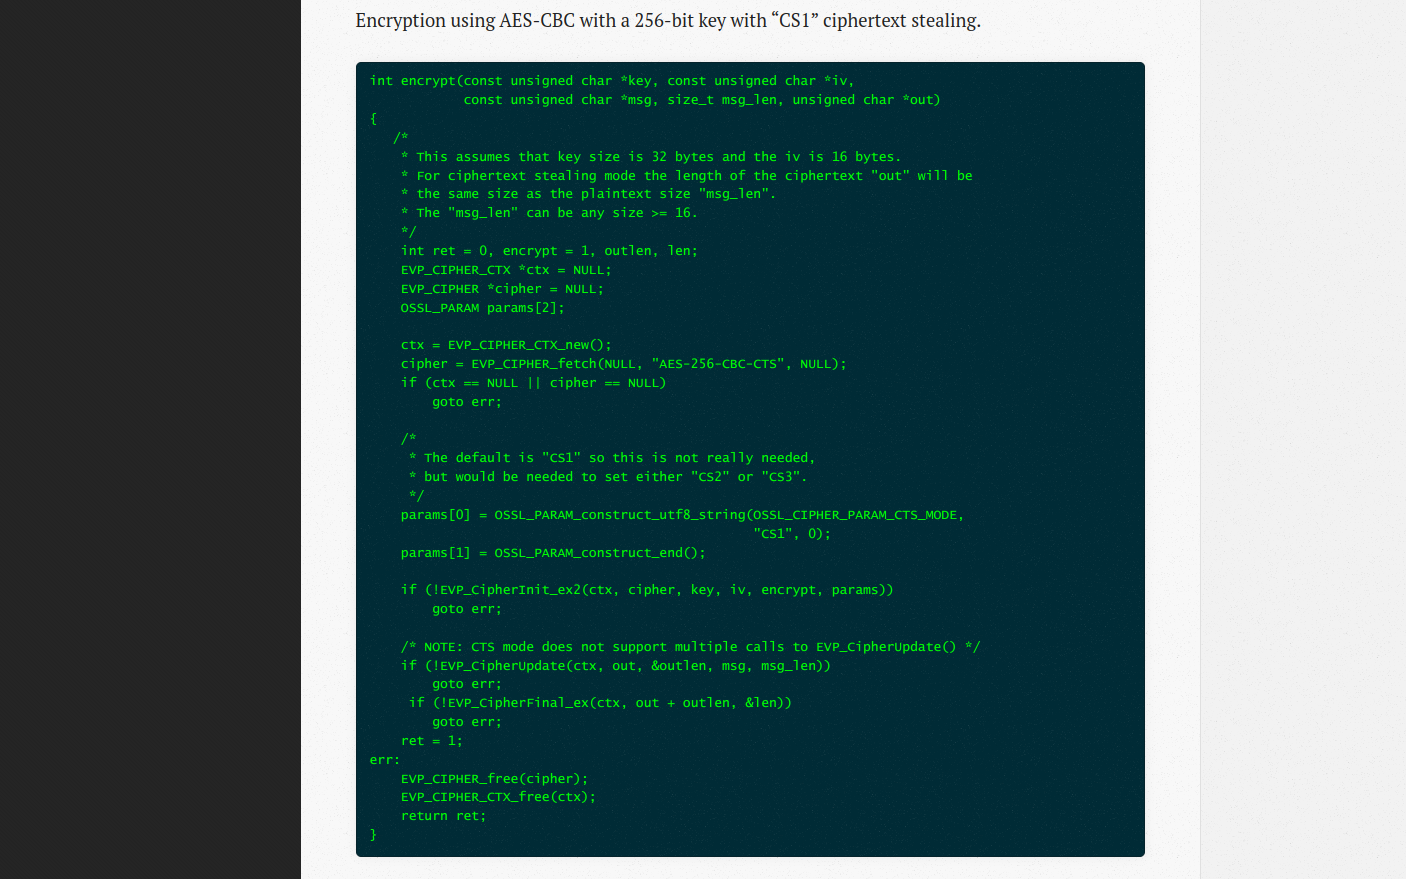
\includegraphics[height=.9\textheight]{assets/opennssl-document.png}
\end{frame}

%%%%%%%%%%%%%%%%%%%%%%%%%%%%%%%%%%%%%%%%%%%%%%%%%%%%%%%%%%%%%%%%%%%%%%%%%%%%%%%%%%%%%%%%%%%%%%%%%%%%%%%%%%%%%%%%%%%%%%%%%%%%%%%%%%%%%%%%%%%%%%%%%%%%%%%%%%%%%%%%%%%%%%%

\begin{frame}{Get Siked!\cite{arstechnica-article}\cite{cryptoeprint:2022/975}}
  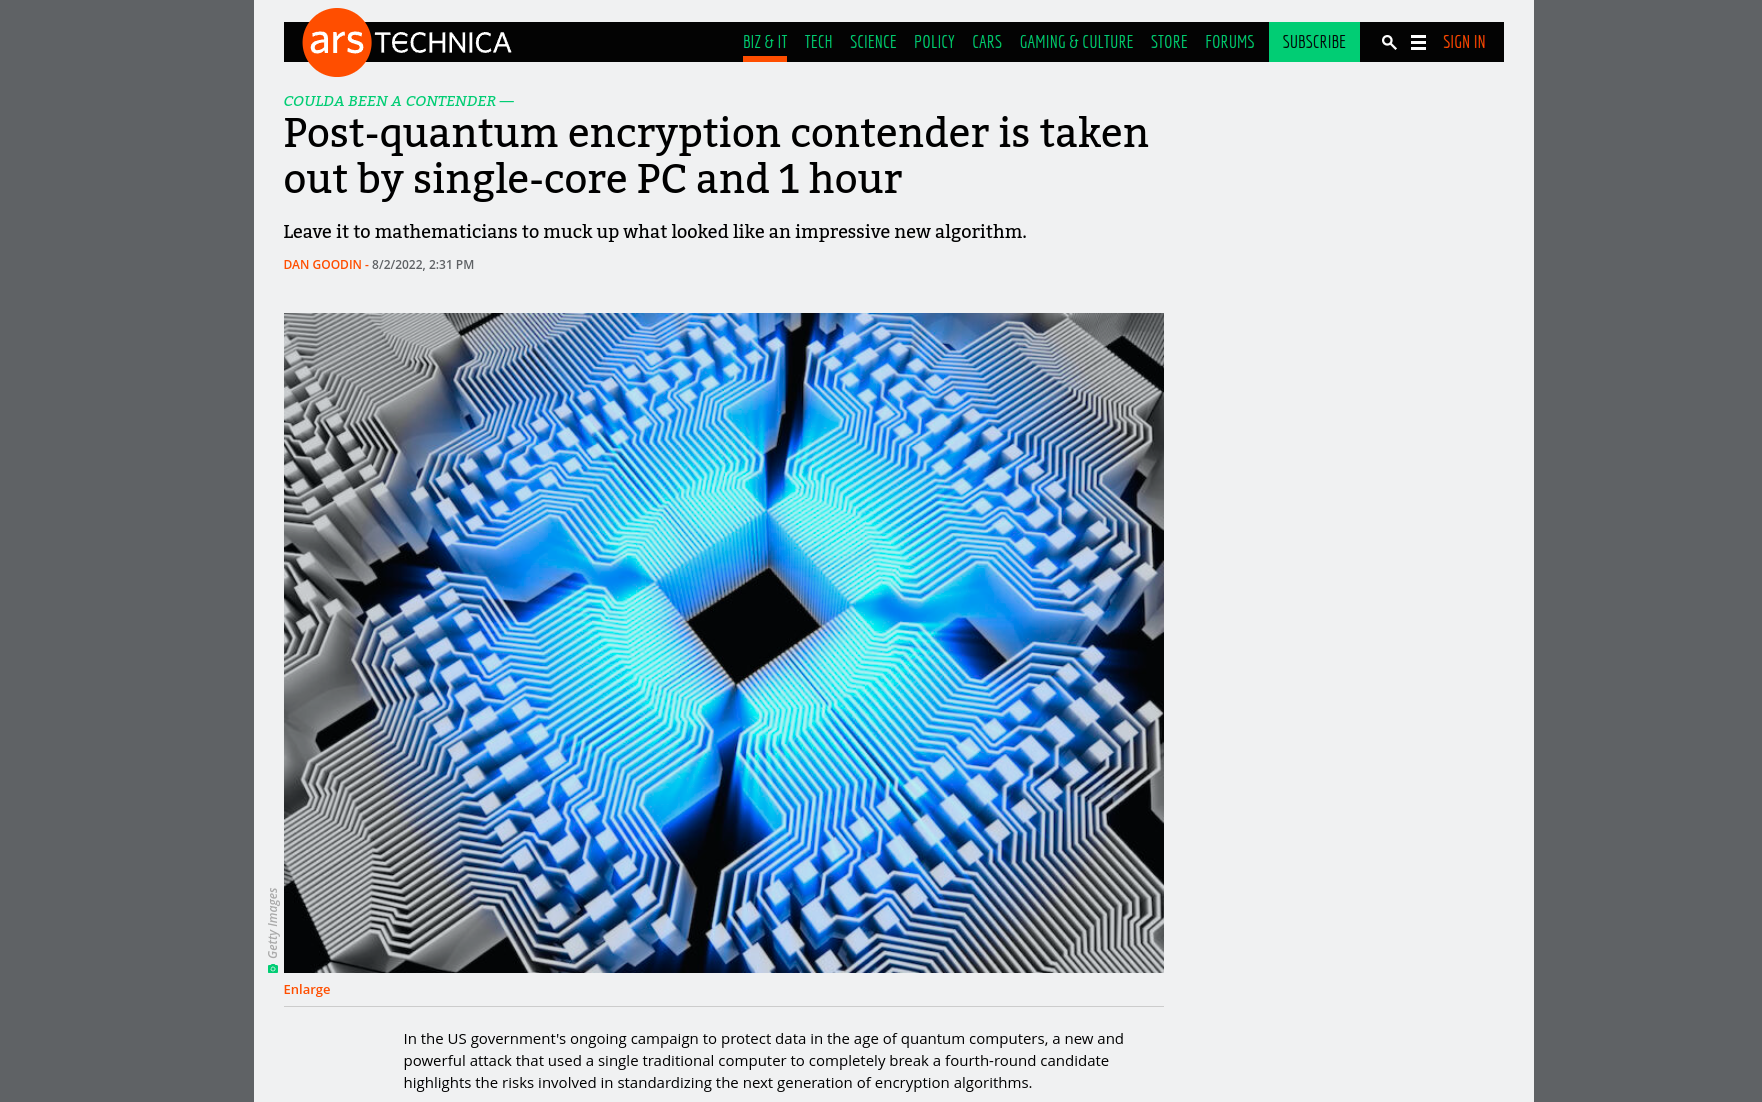
\includegraphics[height=.9\textheight]{assets/ars-headline.png}
\end{frame}

%%%%%%%%%%%%%%%%%%%%%%%%%%%%%%%%%%%%%%%%%%%%%%%%%%%%%%%%%%%%%%%%%%%%%%%%%%%%%%%%%%%%%%%%%%%%%%%%%%%%%%%%%%%%%%%%%%%%%%%%%%%%%%%%%%%%%%%%%%%%%%%%%%%%%%%%%%%%%%%%%%%%%%%

\begin{frame}{Which Ciphers does Rosenpass use?}
  \begin{itemize}
    \item \textbf{Classic McEliece} for Authentication and confidentiality\\
	    (linear code based)
    \item \textbf{Kyber} for Forward Secrecy\\
      (lattice based)
    \item notably both are NIST\footnote{\say{National Institute of Standards and Technology} -- NIST} PQC Standardization Round 3 Finalists\cite{pqc-standardization}
  \end{itemize}
\end{frame}

%%%%%%%%%%%%%%%%%%%%%%%%%%%%%%%%%%%%%%%%%%%%%%%%%%%%%%%%%%%%%%%%%%%%%%%%%%%%%%%%%%%%%%%%%%%%%%%%%%%%%%%%%%%%%%%%%%%%%%%%%%%%%%%%%%%%%%%%%%%%%%%%%%%%%%%%%%%%%%%%%%%%%%%

\begin{frame}{Kyber}
  \framesubtitle{Lattices \& Basis}
\begin{figure}
  \begin{minipage}{.45\textwidth}
    \centering
    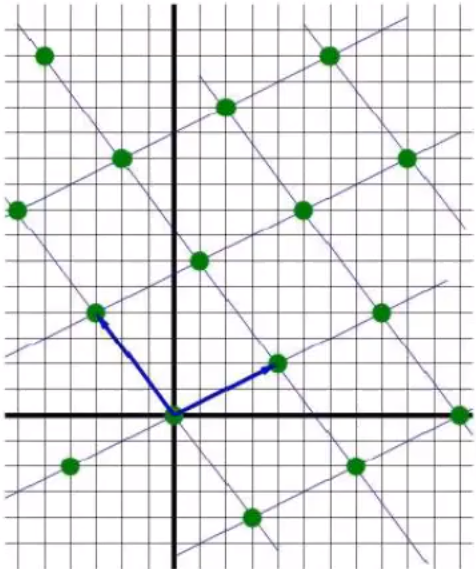
\includegraphics[height=\textwidth]{assets/lattice.png}
  \end{minipage}\hfill
  \begin{minipage}{.45\textwidth}
    \centering
    \(L = {z_1b_1 + z_2b_2} = {\begin{bmatrix}4 & -3\\2 & 4\end{bmatrix} \cdot \begin{bmatrix}z_1\\z_2 \end{bmatrix}}\)
  \end{minipage}
\end{figure}
\end{frame}

%%%%%%%%%%%%%%%%%%%%%%%%%%%%%%%%%%%%%%%%%%%%%%%%%%%%%%%%%%%%%%%%%%%%%%%%%%%%%%%%%%%%%%%%%%%%%%%%%%%%%%%%%%%%%%%%%%%%%%%%%%%%%%%%%%%%%%%%%%%%%%%%%%%%%%%%%%%%%%%%%%%%%%%

\begin{frame}{Kyber}
  \framesubtitle{Lattices -- CVP\footnote{\say{Closest vector problem} -- CVP}}

\begin{figure}
  \begin{minipage}{.45\textwidth}
    \centering
    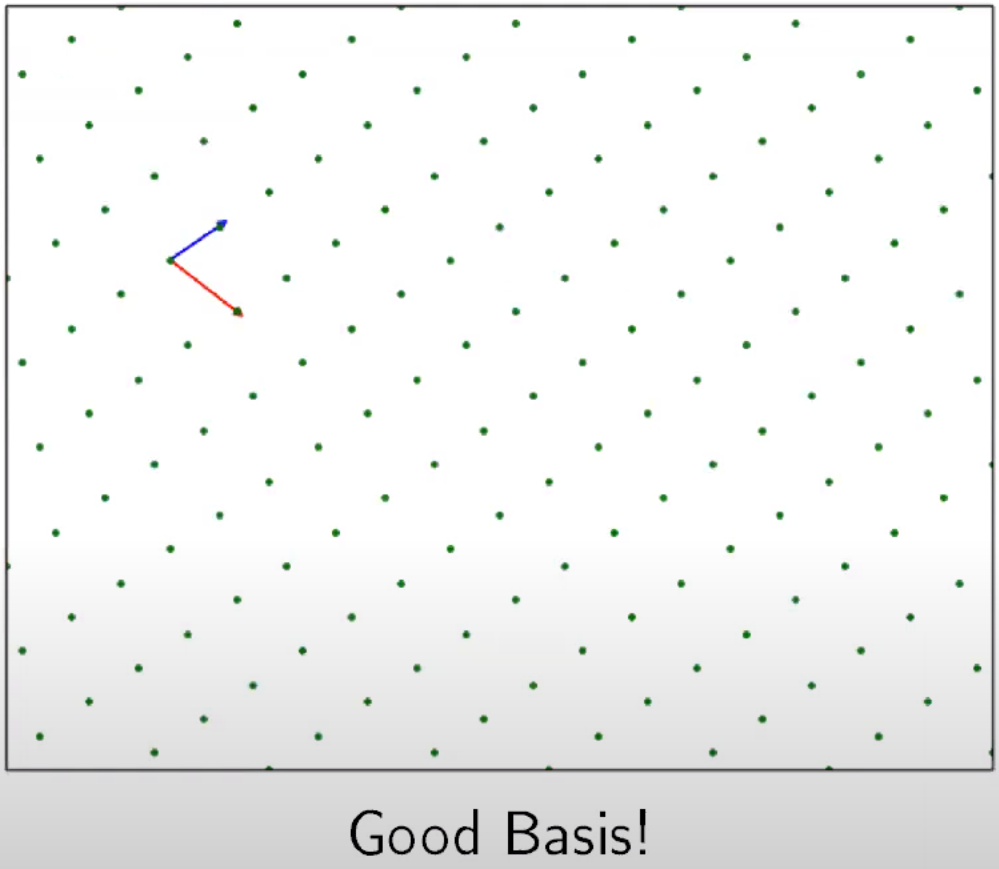
\includegraphics[width=\textwidth]{assets/lattice-good.png}
  \end{minipage}\hfill
  \begin{minipage}{.45\textwidth}
    \centering
    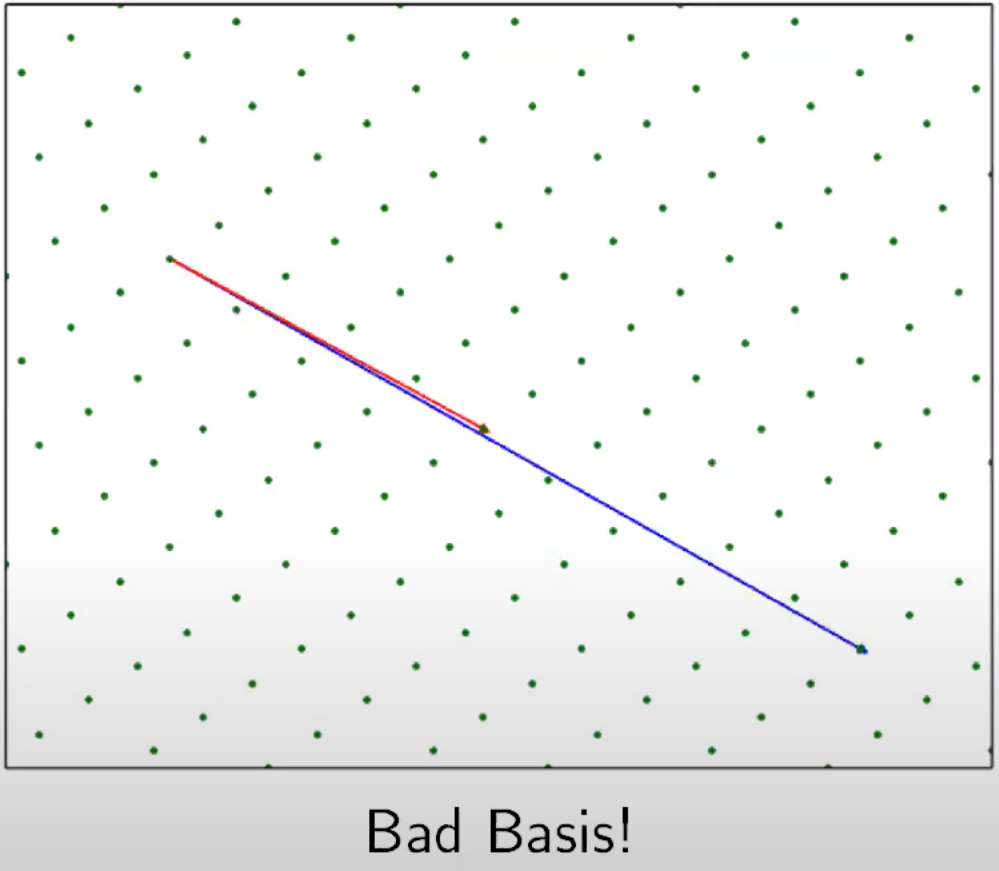
\includegraphics[width=\textwidth]{assets/lattice-bad.png}
  \end{minipage}
\end{figure}
\end{frame}

%%%%%%%%%%%%%%%%%%%%%%%%%%%%%%%%%%%%%%%%%%%%%%%%%%%%%%%%%%%%%%%%%%%%%%%%%%%%%%%%%%%%%%%%%%%%%%%%%%%%%%%%%%%%%%%%%%%%%%%%%%%%%%%%%%%%%%%%%%%%%%%%%%%%%%%%%%%%%%%%%%%%%%%

\begin{frame}{Kyber}
\framesubtitle{LWE}
    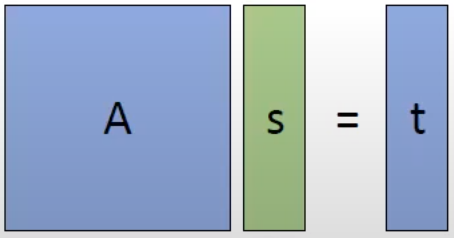
\includegraphics[height=.6\textheight]{assets/matrix.png}
\end{frame}

%%%%%%%%%%%%%%%%%%%%%%%%%%%%%%%%%%%%%%%%%%%%%%%%%%%%%%%%%%%%%%%%%%%%%%%%%%%%%%%%%%%%%%%%%%%%%%%%%%%%%%%%%%%%%%%%%%%%%%%%%%%%%%%%%%%%%%%%%%%%%%%%%%%%%%%%%%%%%%%%%%%%%%%

\begin{frame}{Kyber}
\framesubtitle{LWE\footnote{\say{Learning with Errors} -- LWE}}

\begin{figure}
  \begin{minipage}{.4\textwidth}
    \centering
    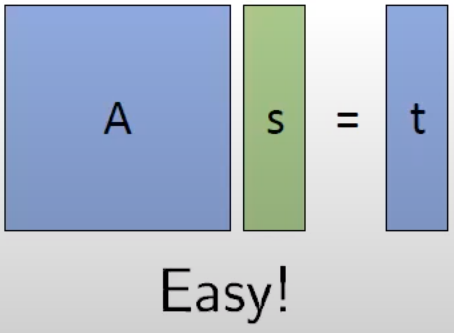
\includegraphics[width=\textwidth]{assets/matrix-easy.png}
  \end{minipage}\hfill
  \begin{minipage}{.4\textwidth}
    \centering
    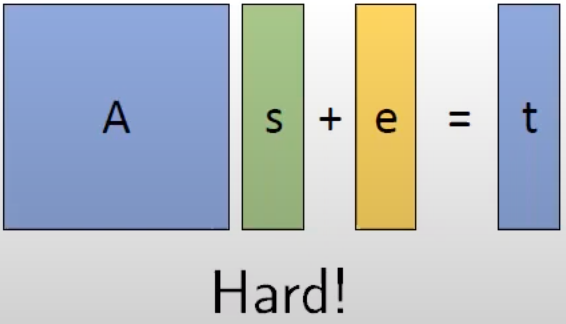
\includegraphics[width=\textwidth]{assets/matrix-hard.png}
  \end{minipage}
\end{figure}
\end{frame}

%%%%%%%%%%%%%%%%%%%%%%%%%%%%%%%%%%%%%%%%%%%%%%%%%%%%%%%%%%%%%%%%%%%%%%%%%%%%%%%%%%%%%%%%%%%%%%%%%%%%%%%%%%%%%%%%%%%%%%%%%%%%%%%%%%%%%%%%%%%%%%%%%%%%%%%%%%%%%%%%%%%%%%%

\begin{frame}{Ciphers available PQC\footnote{\say{Post-quantum cryptography} -- PQC}}
  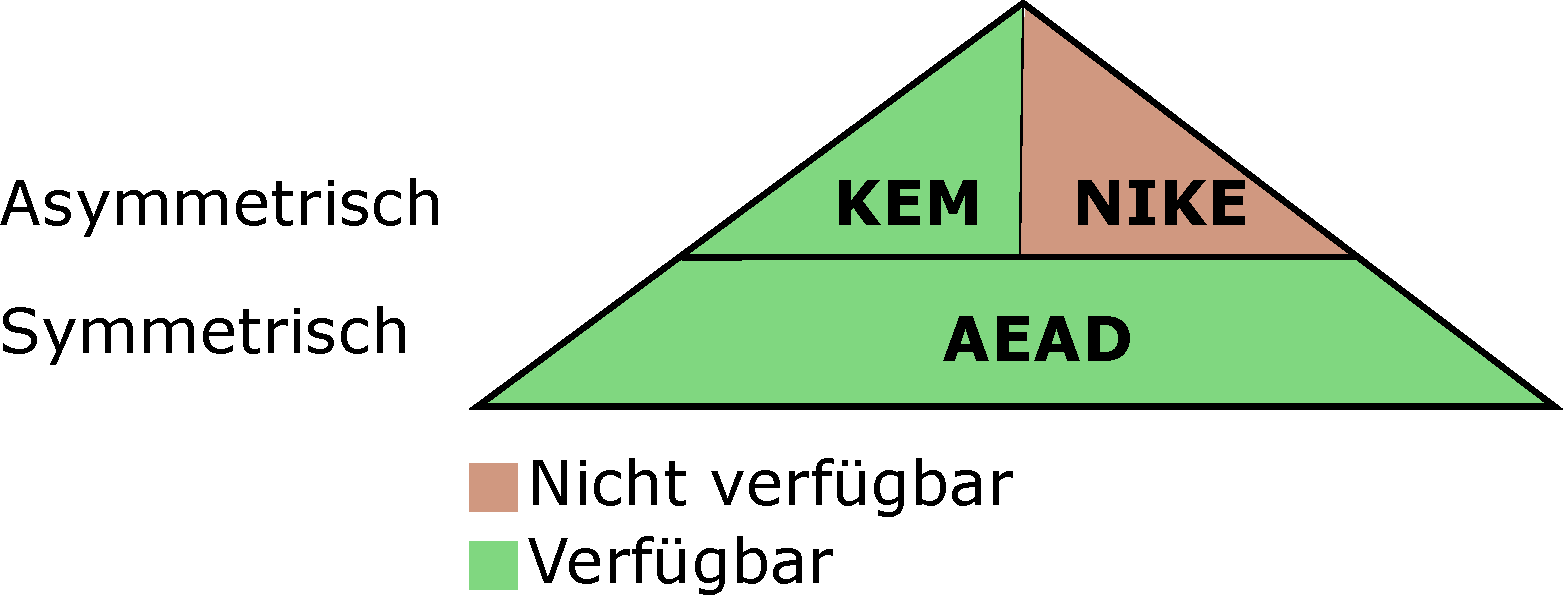
\includegraphics[height=.6\textheight]{graphics/Primitivenpyramide.pdf}
\end{frame}

%%%%%%%%%%%%%%%%%%%%%%%%%%%%%%%%%%%%%%%%%%%%%%%%%%%%%%%%%%%%%%%%%%%%%%%%%%%%%%%%%%%%%%%%%%%%%%%%%%%%%%%%%%%%%%%%%%%%%%%%%%%%%%%%%%%%%%%%%%%%%%%%%%%%%%%%%%%%%%%%%%%%%%%

\begin{frame}[b]{NIKE\footnote{\say{Non-Interactive Key Exchange} -- NIKE}}
\hspace*{-.9\csname beamer@leftmargin\endcsname}\begin{tikzpicture}[
rosenpass-diagram,
  % define multiple syles for consistency
  boxed-node/.style = {draw, rectangle, fill=white, text width = 5em, align = center, minimum height = 1.75em, rounded corners},
  swimming-lane/.style = {very thick},
  message-flow/.style = {-{Stealth[length = 0.5em]}, shorten >= 0.25em, shorten <= 0.25em},
  yscale=.7
]

  % iterate over i, multiply with 1cm, creating a vertical, down moving row of coordinates
  \foreach \i [evaluate=\i as \angle using { \i * 1cm}] in {0,...,5}
    \coordinate (n-\i) at (0,-\i);

  % set two initial nodes, positioned relative to the coordinates
	 \draw[initiator](-1,0) node(initiator){Initiator} coordinate(ini) ++(0,.1)to
		coordinate[pos=.2](spki-y)
		coordinate[pos=.6](spkr-y)
		coordinate[pos=.76](ack-y)+(0,-5) coordinate(result-y);
	  \draw[responder] (1,0) node(responder){Response} coordinate (res)++(0,.1)to +(0,-5);

  % place a text on the intersection of the ini node and the n-1 coordinate
  \node[anchor = east] (sski) at (n-1 -| ini) {(sski, spki) $\leftarrow$ keygen()};

  % place a text on the intersection of the res node and the n-2 coordinate
  \node[anchor = west] (sskr) at (n-2 -| res) {(sskr, spkr) $\leftarrow$ keygen()};

  % place text on below ini and res node on the height of the n-3 coordinate
  \node[anchor = east] (dhi) at (n-4 -| ini) {key $\leftarrow$ dh(sski, spkr)};
  \node[anchor = west] (dhr) at (n-4 -| res) {key $\leftarrow$ dh(sskr, spki)};

  % define the message flows
  \begin{scope}[style = message-flow]
     \draw [request](sski) -- node[above]{spki} (sski -| res);
     \draw [response](n-2 -| ini) -- node[above]{spkr} (n-2 -| res);
  \end{scope}
\end{tikzpicture}\hfill\begingroup\footnotesize
\raisebox{-\baselineskip}{\makebox[4cm][l]{%
	\begin{tikzpicture}[outer sep=1mm]
		\namepart{s=Static,e=Ephemeral}
		\namepart[2cm]{sk=Secret Key,pk=Public Key,ct=Ciphertext}
		\namepart[4cm]{i=Initiator,r=Responder}
		\begin{scope}[decoration={brace,amplitude=3mm},thick]
			\namebraceright{s}{e}
			\namebraceleft{sk}{ct}
			\namebraceright{sk}{ct}
			\namebraceleft{i}{r}
		\end{scope}
\end{tikzpicture}}}
\endgroup
\end{frame}

%%%%%%%%%%%%%%%%%%%%%%%%%%%%%%%%%%%%%%%%%%%%%%%%%%%%%%%%%%%%%%%%%%%%%%%%%%%%%%%%%%%%%%%%%%%%%%%%%%%%%%%%%%%%%%%%%%%%%%%%%%%%%%%%%%%%%%%%%%%%%%%%%%%%%%%%%%%%%%%%%%%%%%%

\begin{frame}[b]{KEM\footnote{\say{Key-Encapsulation Method} -- KEM}\cite{cryptoeprint:2022/1225}}
\hspace*{-.9\csname beamer@leftmargin\endcsname}\begin{tikzpicture}[
rosenpass-diagram,
  % define multiple syles for consistency
  boxed-node/.style = {draw, rectangle, fill=white, text width = 5em, align = center, minimum height = 1.75em, rounded corners},
  swimming-lane/.style = {very thick},
  message-flow/.style = {-{Stealth[length = 0.5em]}, shorten >= 0.25em, shorten <= 0.25em},
  yscale=.8
]

  % iterate over i, multiply with 1cm, creating a vertical, down moving row of coordinates
  \foreach \i [evaluate=\i as \angle using { \i * .8cm}] in {0,...,6}
    \coordinate (n-\i) at (0,-\i);

  % set two initial nodes, positioned relative to the coordinates
		 \draw[initiator](-1,0) node(initiator){Initiator} coordinate(ini) ++(0,.1)to
			coordinate[pos=.2](spki-y)
			coordinate[pos=.6](spkr-y)
			coordinate[pos=.76](ack-y)+(0,-5) coordinate(result-y);
		  \draw[responder] (1,0) node(responder){Response} coordinate (res)++(0,.1)to +(0,-5);
	

  % place a text on the intersection of the res node and the n-2 coordinate
  \node[anchor = west] (sskr) at (n-1 -| res) {(sskr, spkr) $\leftarrow$ keygen()};

  % place a text on the intersection of the res node and the n-2 coordinate
  \node[anchor = east] (sctr) at (n-3 -| ini) {(key, sctr) $\leftarrow$ encaps(spkr)};
  \node[anchor = west] (decapsr) at (n-3 -| res) {key $\leftarrow$ decaps(sctr)};


  % define the message flows
  \begin{scope}[style = message-flow]
     \draw [response](n-1 -| ini) -> node[above]{spkr} (n-1 -| res);
     \draw [request](sctr) -> node[above]{sctr} (sctr -| res);
  \end{scope}
\end{tikzpicture}%
\hfill
\begingroup\footnotesize
\raisebox{-\baselineskip}{%
\makebox[4cm][l]{%
	\begin{tikzpicture}[outer sep=1mm]
		\namepart{s=Static,e=Ephemeral}
		\namepart[2cm]{sk=Secret Key,pk=Public Key,ct=Ciphertext}
		\namepart[4cm]{i=Initiator,r=Responder}
		\begin{scope}[decoration={brace,amplitude=3mm},thick]
			\namebraceright{s}{e}
			\namebraceleft{sk}{ct}
			\namebraceright{sk}{ct}
			\namebraceleft{i}{r}
		\end{scope}
\end{tikzpicture}}}
\endgroup
\end{frame}

%%%%%%%%%%%%%%%%%%%%%%%%%%%%%%%%%%%%%%%%%%%%%%%%%%%%%%%%%%%%%%%%%%%%%%%%%%%%%%%%%%%%%%%%%%%%%%%%%%%%%%%%%%%%%%%%%%%%%%%%%%%%%%%%%%%%%%%%%%%%%%%%%%%%%%%%%%%%%%%%%%%%%%%

\begin{frame}{Rosenpass Key Exchange}
  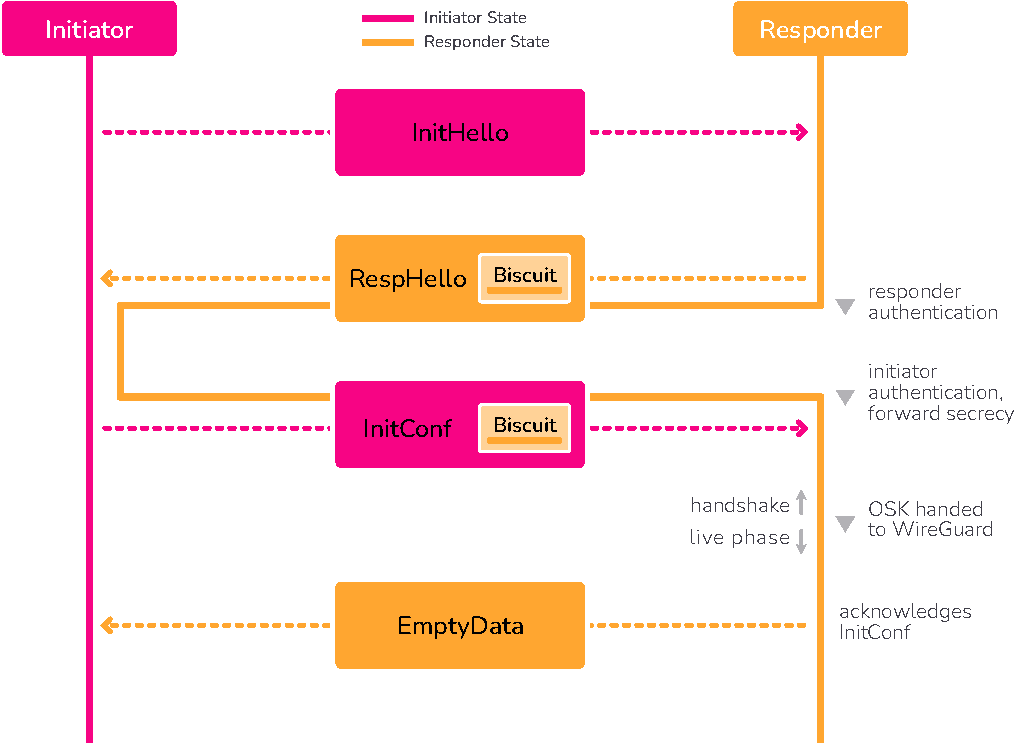
\includegraphics[height=.9\textheight]{graphics/rosenpass-wp-key-exchange-protocol-rgb.pdf}
\end{frame}

%%%%%%%%%%%%%%%%%%%%%%%%%%%%%%%%%%%%%%%%%%%%%%%%%%%%%%%%%%%%%%%%%%%%%%%%%%%%%%%%%%%%%%%%%%%%%%%%%%%%%%%%%%%%%%%%%%%%%%%%%%%%%%%%%%%%%%%%%%%%%%%%%%%%%%%%%%%%%%%%%%%%%%%

\begin{frame}{Wireguard Integration\cite{cryptoeprint:2016/1017}}
  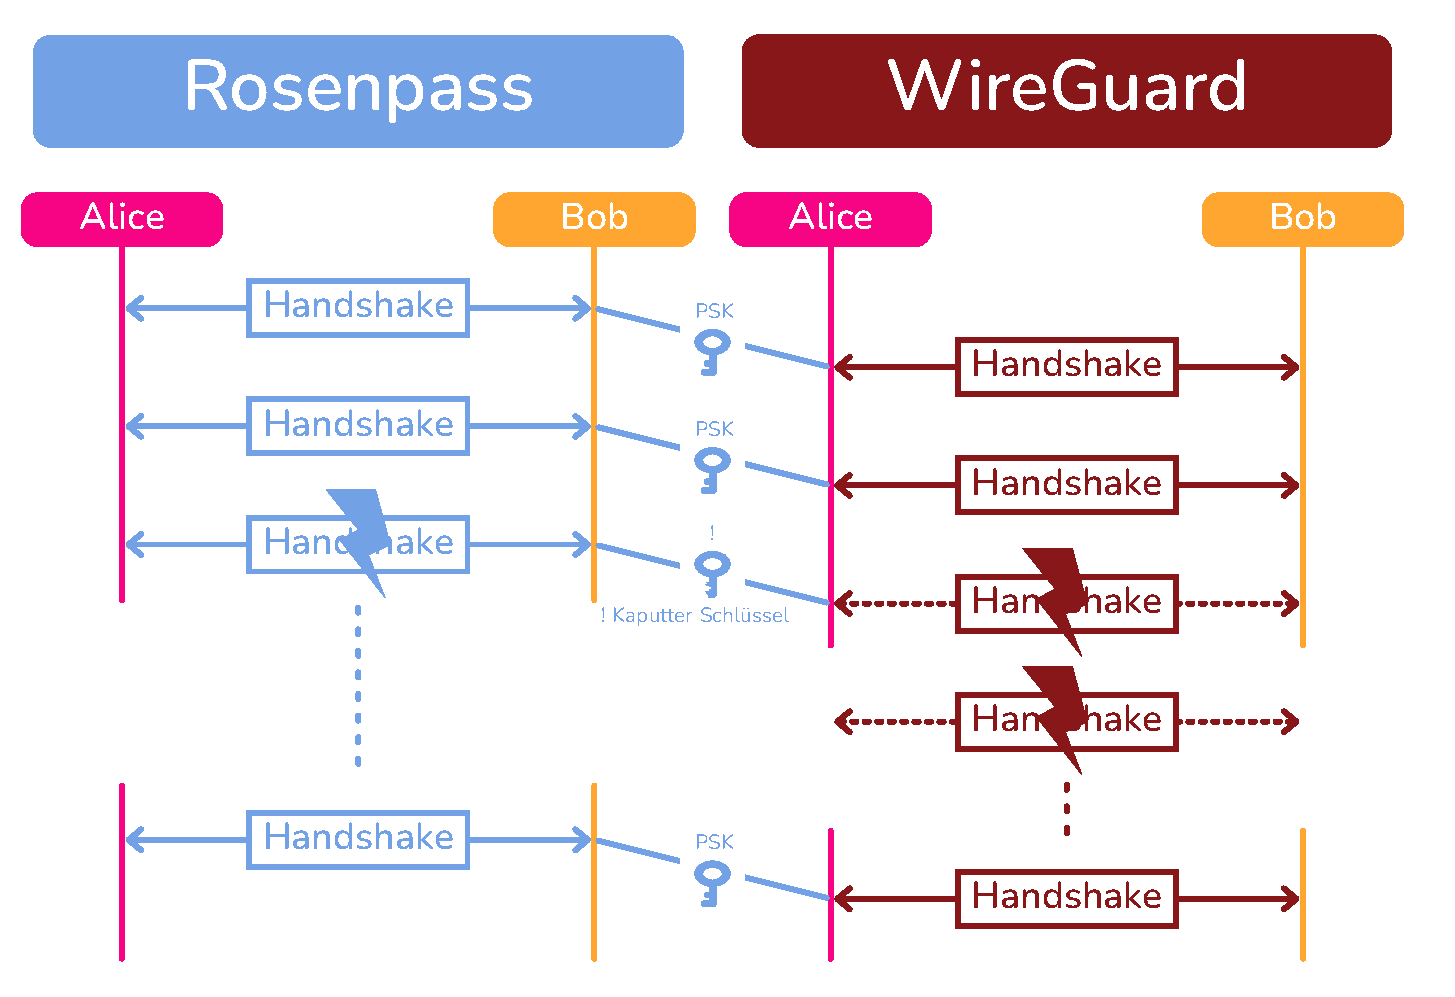
\includegraphics[height=.9\textheight]{assets/rosenpass-wireguard.png}
\end{frame}

%%%%%%%%%%%%%%%%%%%%%%%%%%%%%%%%%%%%%%%%%%%%%%%%%%%%%%%%%%%%%%%%%%%%%%%%%%%%%%%%%%%%%%%%%%%%%%%%%%%%%%%%%%%%%%%%%%%%%%%%%%%%%%%%%%%%%%%%%%%%%%%%%%%%%%%%%%%%%%%%%%%%%%%

\begin{frame}
\centering

\includegraphics[width=.4\linewidth]{RosenPass-Logo}
\end{frame}

%%%%%%%%%%%%%%%%%%%%%%%%%%%%%%%%%%%%%%%%%%%%%%%%%%%%%%%%%%%%%%%%%%%%%%%%%%%%%%%%%%%%%%%%%%%%%%%%%%%%%%%%%%%%%%%%%%%%%%%%%%%%%%%%%%%%%%%%%%%%%%%%%%%%%%%%%%%%%%%%%%%%%%%

\begin{frame}{Sources}
  \printbibliography
\end{frame}

\edef\totalcontentframes{\theframenumber}

%%%%%%%%%%%%%%%%%%%%%%%%%%%%%%%%%%%%%%%%%%%%%%%%%%%%%%%%%%%%%%%%%%%%%%%%%%%%%%%%%%%%%%%%%%%%%%%%%%%%%%%%%%%%%%%%%%%%%%%%%%%%%%%%%%%%%%%%%%%%%%%%%%%%%%%%%%%%%%%%%%%%%%%

\begin{frame}{Question 1:}
\begin{itemize}
  \item Do you think Rosenpass has a future if PQ Ciphers establish themselves?
  \item 
\end{itemize}
\end{frame}

%%%%%%%%%%%%%%%%%%%%%%%%%%%%%%%%%%%%%%%%%%%%%%%%%%%%%%%%%%%%%%%%%%%%%%%%%%%%%%%%%%%%%%%%%%%%%%%%%%%%%%%%%%%%%%%%%%%%%%%%%%%%%%%%%%%%%%%%%%%%%%%%%%%%%%%%%%%%%%%%%%%%%%%

\begin{frame}{Question 1:}
\begin{itemize}
  \item Do you think Rosenpass has a future if PQ Ciphers establish themselves?
  \item Hint: 'Technical Dept'
\end{itemize}
\end{frame}

%%%%%%%%%%%%%%%%%%%%%%%%%%%%%%%%%%%%%%%%%%%%%%%%%%%%%%%%%%%%%%%%%%%%%%%%%%%%%%%%%%%%%%%%%%%%%%%%%%%%%%%%%%%%%%%%%%%%%%%%%%%%%%%%%%%%%%%%%%%%%%%%%%%%%%%%%%%%%%%%%%%%%%%

\begin{frame}{Question 2:}
\begin{itemize}
  \item The Rosenpass developers may allow you to choose your own ciphers in the future.
    Why would they \textbf{not} enable this?
  \item 
\end{itemize}
\end{frame}

%%%%%%%%%%%%%%%%%%%%%%%%%%%%%%%%%%%%%%%%%%%%%%%%%%%%%%%%%%%%%%%%%%%%%%%%%%%%%%%%%%%%%%%%%%%%%%%%%%%%%%%%%%%%%%%%%%%%%%%%%%%%%%%%%%%%%%%%%%%%%%%%%%%%%%%%%%%%%%%%%%%%%%%

\begin{frame}{Question 2:}
\begin{itemize}
  \item The Rosenpass developers may allow you to choose your own ciphers in the future.
    Why would they \textbf{not} enable this?
  \item Hint: They definitely won't allow for \textbf{dynamic negotiation} of ciphers between initiator and responder.
\end{itemize}
\end{frame}

%%%%%%%%%%%%%%%%%%%%%%%%%%%%%%%%%%%%%%%%%%%%%%%%%%%%%%%%%%%%%%%%%%%%%%%%%%%%%%%%%%%%%%%%%%%%%%%%%%%%%%%%%%%%%%%%%%%%%%%%%%%%%%%%%%%%%%%%%%%%%%%%%%%%%%%%%%%%%%%%%%%%%%%

\begin{frame}{Question 3:}
\begin{itemize}
  \item Despite this, why would Administrators 'choose' to pick different cipers?
  \item 
\end{itemize}
\end{frame}

%%%%%%%%%%%%%%%%%%%%%%%%%%%%%%%%%%%%%%%%%%%%%%%%%%%%%%%%%%%%%%%%%%%%%%%%%%%%%%%%%%%%%%%%%%%%%%%%%%%%%%%%%%%%%%%%%%%%%%%%%%%%%%%%%%%%%%%%%%%%%%%%%%%%%%%%%%%%%%%%%%%%%%%

\begin{frame}{Question 3:}
\begin{itemize}
  \item Despite this, why would Administrators 'choose' to pick different cipers?
  \item Hint: National Institute of Standards and Technology (NIST)
\end{itemize}
\end{frame}

%%%%%%%%%%%%%%%%%%%%%%%%%%%%%%%%%%%%%%%%%%%%%%%%%%%%%%%%%%%%%%%%%%%%%%%%%%%%%%%%%%%%%%%%%%%%%%%%%%%%%%%%%%%%%%%%%%%%%%%%%%%%%%%%%%%%%%%%%%%%%%%%%%%%%%%%%%%%%%%%%%%%%%%
% End Document
%%%%%%%%%%%%%%%%%%%%%%%%%%%%%%%%%%%%%%%%%%%%%%%%%%%%%%%%%%%%%%%%%%%%%%%%%%%%%%%%%%%%%%%%%%%%%%%%%%%%%%%%%%%%%%%%%%%%%%%%%%%%%%%%%%%%%%%%%%%%%%%%%%%%%%%%%%%%%%%%%%%%%%%

\setcounter{framenumber}{\totalcontentframes}

\end{document}
